\section{Experimentación}
Los primeros dos experimentos que veremos, se centran en el tiempo de ejecución de los procesos. Dichos experimentos tienen como finalidad estudiar como influye la cantidad de frames del video y la cantidad de frames a generar en el tiempo de ejecución, y si un video con mucho movimiento implica mayor tiempo de procesamiento que uno estático.\\

\subsection{Experimentación Temporal}

Como video de prueba, utilizamos una escena de un partido de futbol donde hay gran cantidad de movimiento y un video cuyos frames son todos blancos.\\

En el primer experimento medimos el tiempo de generación de frames aumentando en cada medición la cantidad de frames a generar en el video de futbol.

%grafico donde la cantidad de frames a generar aumenta
\begin{wrapfigure}{r}{0.6\textwidth}
  \vspace{-20pt}
  \begin{center}
    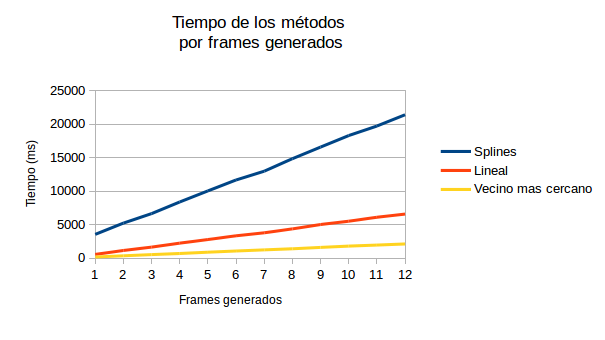
\includegraphics[scale= 0.6]{imagenes/aumentandoFramesToAdd.png}
  \end{center}
  \vspace{-10pt}
  \vspace{-10pt}
\end{wrapfigure}

Como vemos en el gráfico, el tiempo de procesamiento es lineal, esto es debido a que en cada iteración aumentamos la cantidad de frames a generar. Era de esperarse que un método como splines resultara ser el que más tarde en realizar su tarea, dado que realiza más operaciones que los otros métodos. \\

Por otro lado, realizamos una medición de tiempos con el mismo video, donde la cantidad de frames a generar es 1,   las dimensiones de los frames son fijas, y lo que variamos fue la cantidad de frames del video de entrada, aumentándolo de a 8 frames en cada medición. Para el video con movimiento, tomamos un segmento de un video largo tomando cada vez más frames, siempre desde el mismo frame original. Obtuvimos los siguientes resultados:


\begin{figure}[h!]
  \centering
    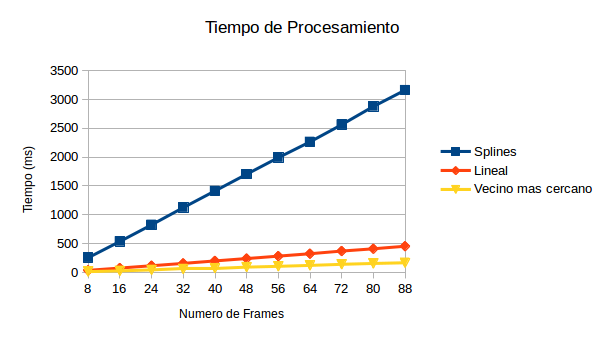
\includegraphics[scale= 0.6]{imagenes/aumentandoFramesMessi.png}
  \caption{Tiempo de Procesamiento agregando 1 frame aumentando la cantidad de frames originales}
\end{figure}

Los resultados que obtuvimos fueron lineales, como en el experimento anterior, con lo cual concluimos que la complejidad no depende únicamente de la cantidad de frames a generar, sino también de la cantidad de frames de entrada.\\


Intuitivamente el tiempo de procesamiento para cada método no debería variar si el video de prueba tiene gran movimiento o no, es decir, si hay mucha variacón del color de pixel entre frame y frame. Intuimos esto porque las operaciones que dependen del valor de un pixel son de tiempo constante (multiplicaciones, divisiones, sumas, restas y asignaciones). En particular, el video de prueba del experimento anterior, tenía una escena donde habia mucho movimiento, y esto no se reflejó en la medición temporal. \\

Por otro lado, tomamos los tiempo de procesamiento para un video del mismo ancho y largo que el video anterior, donde todos los frames eran blancos (todos los pixeles valen 255) tomando en cada medicion la misma cantidad de frames para poder ver efectivamente si los tiempos obtenidos eran menores, mayores o iguales. Los resultados obtenidos fueron muy parecidos al otro video, por lo que decidimos graficarlo tomando los tiempos del video con movimiento dividido el tiempo del video en blanco.

\begin{wrapfigure}{r}{0.6\textwidth}
  \vspace{-20pt}
  \begin{center}
    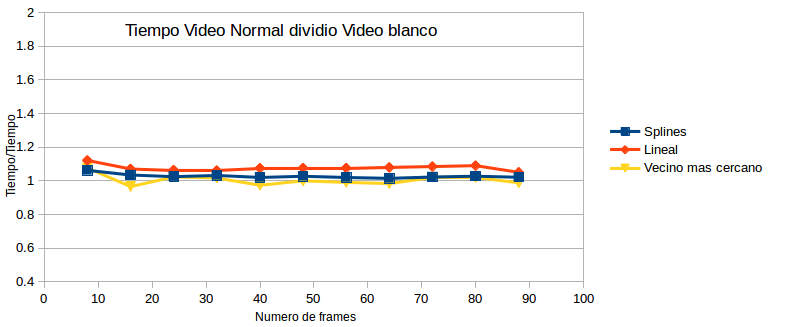
\includegraphics[scale= 0.6]{imagenes/aumentandoFramesMessiSobreWhite.png}
  \end{center}
  \vspace{-10pt}
  \vspace{-10pt}
\end{wrapfigure}

La mayor diferencia de tiempo entre ambos videos surgió en el método de splines. A pesar de no ser un tiempo significativamente distinto, creemos que la razón de que el tiempo sea ligeramente mayor en el video con movimiento radica en que los coeficientes de los polinomios obtenidos para el video en blanco son cero mientras que esto no sucede así para el otro video, haciendo que la evaluacion del polinomio sea más rápida.

\subsection{Experimentación Cualitativa}

En esta sección analizamos las mediciones con el error cuadrático medio (ECM) y el Peak Signal to Noise Ratio (PSNR) y analizamos el impacto de los aspectos cualitativos de los vídeos en los métodos propuestos. \\

En el siguiente experimento, tomamos un video y le quitamos frames, para luego generarlos. Estudiamos como varía dicho índice comparando los frames originales que quitamos y los frames generados que los reemplazan. Utilizamos un video con cambios de cámara repentinos para poder ver como se comportan los métodos y ver el PSNR obtenido en esos cortes. Para esto, utilizamos un segmento del video $Gangnam Style$ que posee estas cualidades.
Los resultados que obtuvimos fueron los siguientes:


\begin{figure}[h!]
  \caption{Gráfico del ECM comparando contra frames originales}
  \centering
    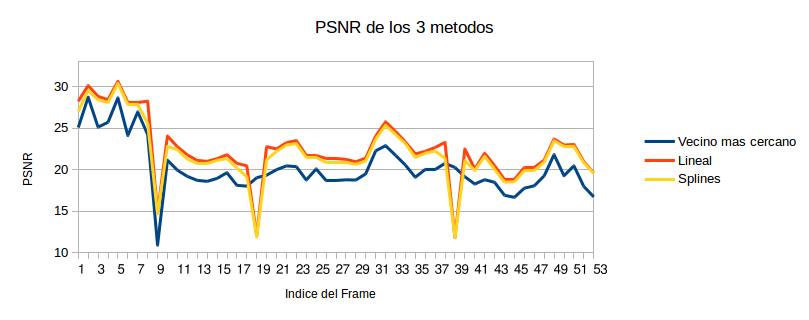
\includegraphics[scale=0.75]{imagenes/PSNRGangnam.png}
\end{figure}

Los picos inferiores del gráfico se corresponden con los frames donde ocurre un cambio de toma brusco. El pico más bajo corresponde al método del vecino más cercano, como esperabamos. Sin embargo, no sucede lo mismo con los otros dos picos. Esto se debe a que para esos frames, el algoritmo seleccinó los frames posteriores al cambio de toma, teniendo así una menor diferencia que los otros métodos.

%grafico de medicion de ecm con 
% \begin{wrapfigure}{r}{0.6\textwidth}
%   \vspace{-20pt}
%   \begin{center}
%     \includegraphics[scale= 0.6]{imagenes/.png}
%   \end{center}
%   \vspace{-10pt}
%   \vspace{-10pt}
% \end{wrapfigure}






